%!TEX root = ../main.tex

%!TEX root = ../main.tex

\RequirePackage{bibentry}
\makeatletter\let\saved@bibitem\@bibitem\makeatother

\documentclass{beamer}
\makeatletter\let\@bibitem\saved@bibitem\makeatother

\renewcommand{\baselinestretch}{1.2}\normalsize
\usetheme{default}
\setbeamertemplate{navigation symbols}{}
\setbeamertemplate{footline}[frame number]

\usepackage{verbatim}
\usepackage{etex}

% BIBLIOGRAPHY APACITE
\usepackage[apaciteclassic]{apacite}
\usepackage{notoccite}
\usepackage{bibentry}
\usepackage{pdfpages}

% MATHEMATICS AND FONTS
\DeclareMathOperator*{\argmin}{arg\,min}
\DeclareMathOperator*{\argmax}{arg\,max}

\renewcommand{\vec}[1]{\mathbf{#1}}

\usepackage{amsfonts}
\usepackage{amsmath}
\usepackage{amssymb}
\usepackage{bbm}
\usepackage{algpseudocode}
\usepackage{setspace}

\usepackage{arev}
\usepackage[latin1]{inputenc}
\usepackage[T1]{fontenc}

\definecolor{darkblue}{rgb}{0,.35,.62}
\definecolor{lightblue}{rgb}{0.8,0.85,1}
\definecolor{lightgrey}{gray}{0.1}	%Farben mischen
\definecolor{Gray}{gray}{0.9}
\definecolor{mplorange}{HTML}{FF7F0E}
\definecolor{mplred}{HTML}{D62728}
\definecolor{mplblue}{HTML}{1F77B4}
\definecolor{mplgreen}{HTML}{2CA02C}

% GRAPHS
\usepackage{graphicx}
\usepackage{subfig}
\usepackage{caption}
\graphicspath{{material/}}
\usepackage{relsize}
\usepackage{lscape}
\usepackage{fancybox}
\usepackage{epstopdf}


% TABLES AND OTHER ENVIRONMENTS
\usepackage{tabularx}
\usepackage{longtable}
\usepackage{booktabs}
\usepackage{color,colortbl}
\usepackage{threeparttable}

\usepackage{enumerate}

\usepackage{fix-cm}

\usepackage{bookmark}
\usepackage{hyperref}
\hypersetup{colorlinks=true,urlcolor=blue,citecolor=black}


\usepackage{tikz}
\tikzset{
	treenode/.style = {shape=rectangle, rounded corners,
		draw, align=center,
		top color=white, bottom color=blue!20},
	root/.style     = {treenode, font=\Large, bottom color=red!30},
	env/.style      = {treenode, font=\ttfamily\normalsize},
	dummy/.style    = {circle,draw}
}
%\usepackage{cmbright}
\def\newblock{\hskip .11em plus .33em minus .07em}
\newcommand{\bs}{\boldsymbol}
\newcommand{\N}{\mathbb{N}}
\newcommand{\cov}{\mathrm{cov}\thin}
\newcommand{\thin}{\thinspace}
\newcommand{\thick}{\thickspace}
\newcommand{\Lim}[1]{\raisebox{0.5ex}{\scalebox{0.8}{$\displaystyle \lim_{#1}\;$}}}

\newcommand{\vect}[1]{\mathbf{#1}}
\newcommand{\myfrac}[3][0pt]{\genfrac{}{}{}{}{\raisebox{#1}{$#2$}}{\raisebox{-#1}{$#3$}}}
\newcommand{\U}{\mathrm{U}}	%Uniform Distribution
\newcommand{\D}{\mathrm{D}}	%Dirichlet Distribution
\newcommand{\W}{\mathrm{W}}	%Wishart Distribution
\newcommand{\E}{\mathrm{E}}		%Expectation
\newcommand{\Prob}{\mbox{Pr}}		%Expectation
\newcommand{\Iden}{\mathbb{I}}	%Identity Matrix
\newcommand{\Ind}{\mathrm{I}}	%Indicator Function
\newcommand{\Tau}{\mathcal{T}\thin}

\newcommand{\var}{\mathrm{var}\thin}
\newcommand{\plim}{\mathrm{plim}\thin}
\newcommand\indep{\protect\mathpalette{\protect\independenT}{\perp}}
\def\independenT#1#2{\mathrel{\rlap{$#1#2$}\mkern5mu{#1#2}}}
\newcommand{\notindep}{\ensuremath{\perp\!\!\!\!\!\!\diagup\!\!\!\!\!\!\perp}}%

\newcommand{\mc}{\multicolumn}

\newcommand{\ph}{\phantom}
% weitere Optionen:
% secbar: Gliederung im Kopf, nur sections (alternativ zu subsecbar)
% handout: Produktion von Handouts, keine Animationen
\definecolor{darkblue}{rgb}{0,.35,.62}
\definecolor{lightblue}{rgb}{0.8,0.85,1}
\definecolor{lightgrey}{gray}{0.1}	%Farben mischen

%	kbordermatrix options

\makeatletter
\newcommand{\vast}{\bBigg@{4}}
\newcommand{\Vast}{\bBigg@{5}}
\makeatother
\newcommand{\indicator}[1]{\mathbbm{1}{\left\{ {#1} \right\} }}
\newcommand{\indic}{1{\hskip -2.5 pt}\hbox{1} }


\definecolor{lightgrey}{gray}{0.90}	%Farben mischen
\definecolor{grey}{gray}{0.85}
\definecolor{darkgrey}{gray}{0.65}
\definecolor{lightblue}{rgb}{0.8,0.85,1}

\renewcommand{\arraystretch}{1.5}


\usepackage{tikz}
\usetikzlibrary{trees,shapes,arrows,decorations.pathmorphing,backgrounds,positioning,fit,petri}
\renewcommand*{\familydefault}{\sfdefault}

\tikzset{forestyle/.style = {rectangle, thick, minimum width = 5cm, minimum height = 0.5cm, text width = 4.5cm, outer sep = 1mm},
	pre/.style={<-, shorten <=1pt, >=stealth, ultra thick},
	extend/.style={<-,dashed, shorten <=1pt, >=stealth, ultra thick}}
\captionsetup[subfigure]{labelformat=empty}


\newcommand{\beginbackup}{
	\newcounter{framenumbervorappendix}
	\setcounter{framenumbervorappendix}{\value{framenumber}}
}
\newcommand{\backupend}{
	\addtocounter{framenumbervorappendix}{-\value{framenumber}}
	\addtocounter{framenumber}{\value{framenumbervorappendix}}
}


% Begin Full Justification ---------------------------------------------------------

\usepackage{ragged2e}
% \usepackage{etoolbox}
\usepackage{lipsum}
\makeatletter
\renewcommand{\itemize}[1][]{%
	\beamer@ifempty{#1}{}{\def\beamer@defaultospec{#1}}%
	\ifnum \@itemdepth >2\relax\@toodeep\else
	\advance\@itemdepth\@ne
	\beamer@computepref\@itemdepth% sets \beameritemnestingprefix
	\usebeamerfont{itemize/enumerate \beameritemnestingprefix body}%
	\usebeamercolor[fg]{itemize/enumerate \beameritemnestingprefix body}%
	\usebeamertemplate{itemize/enumerate \beameritemnestingprefix body begin}%
	\list
	{\usebeamertemplate{itemize \beameritemnestingprefix item}}
	{\def\makelabel##1{%
			{%
				\hss\llap{{%
						\usebeamerfont*{itemize \beameritemnestingprefix item}%
						\usebeamercolor[fg]{itemize \beameritemnestingprefix item}##1}}%
			}%
		}%
	}
	\fi%
	\beamer@cramped%
	\justifying% NEW
	%\raggedright% ORIGINAL
	\beamer@firstlineitemizeunskip%
}

\justifying

% \apptocmd{\frame}{\justifying}{}{}

\usepackage{array}
\newcolumntype{L}[1]{>{\raggedright\let\newline\\\arraybackslash\hspace{0pt}}m{#1}}
\newcolumntype{C}[1]{>{\centering\let\newline\\\arraybackslash\hspace{0pt}}m{#1}}
\newcolumntype{R}[1]{>{\raggedleft\let\newline\\\arraybackslash\hspace{0pt}}m{#1}}



% End Full Justification ------------------------------------------------------------



\title{Generalized Roy Model}
\author{\textbf{Philipp Eisenhauer}}
\date{\parbox{\linewidth}{\centering%
  \ldots{} background material available at \endgraf
 {\urlstyle{same}\url{{https://github.com/policyMetrics/talks}}}}}



\let\otp\titlepage
%\renewcommand{\titlepage}{\otp\addtocounter{framenumber}{-1}}


\begin{document}
\begin{frame}
\maketitle
\end{frame}

% \section{Overview on the Generalized Roy Model}\label{overview-on-the-generalized-roy-model}
%\begin{frame}
%\frametitle{Overview on the Generalized Roy Model}
 %\centering
%\ldots{} background material available at \\ https://github.com/policyMetrics/talks


\begin{frame}
%\subsubsection{Policy Evaluation Tasks}\label{policy-evaluation-tasks}
\frametitle{Policy Evaluation Tasks}
\textbf{Heckman (2008) defines three policy evaluation tasks:}

\begin{itemize}
\item
  Evaluating the impact of historical interventions on outcomes
  including their impact in terms of well-being of the treated and the
  society at large.
\item
  Forecasting the impact of historical interventions implemented in one
  environment in other environments, including their impact in terms of
  well-being.
\item
  Forecasting the impacts of interventions never historically
  experienced to various environments, including their impact on
  well-being.
\end{itemize}

\end{frame}


\begin{frame}
%\subsection{The Generalized Roy Model}\label{the-generalized-roy-model}
\frametitle{The Generalized Roy Model}

\begin{align*}
\textbf{Potential Outcomes} &\qquad \textbf{Cost} \\
Y_1 = \mu_1(X) + U_1      &\qquad C = \mu_D(Z) + U_C \\
Y_0 = \mu_0(X) + U_0      &\qquad \\
    & \\
\textbf{Observed Outcomes } &\qquad \textbf{Choice} \\
Y = D Y_1 + (1 - D)Y_0 &\qquad S = Y_1 - Y_0 - C \\
                       &\qquad D = \mathrm{I}[S > 0] \\
\end{align*}

\end{frame}


\begin{frame}
\frametitle{The Generalized Roy Model}
\textbf{Conventional Notation}
%\subsubsection{Conventional Notation}\label{conventional-notation}

\begin{align*}
Y = \alpha + \beta D + \epsilon,
\end{align*}
where
\begin{align*}
\alpha &= \mu_0(X)  \\
\beta  & = (Y_1 - Y_0) =\mu_1(X) - \mu_0(X)  + (U_1 - U_0)\\
\epsilon & =U_0
\end{align*}

\end{frame}


\begin{frame}
\frametitle{Econometric Problems}
%\subsubsection{Econometric Problems}\label{econometric-problems}

\begin{itemize}
\item
  \textbf{Evaluation Problem:} We only observe an individual in either
  the treated or untreated state.
\item
  \textbf{Selection Problem:} Individuals that select into treatment
  different from those that do not.
\end{itemize}

\end{frame}


\begin{frame}
%\subsubsection{Evaluation Problem}\label{evaluation-problem}
\frametitle{Econometric Problems}

Observed outcome for individual \(i\):

\begin{align*}
Y_i = Y_{0i} + D_i (Y_{1i} - Y_{0i}) =
\begin{cases}
Y_{1i} & \text{if}\quad D_i = 1 \\
Y_{0i} & \text{if}\quad D_i = 0 \\
\end{cases}
\end{align*}

\end{frame}


\begin{frame}
\frametitle{Econometric Problems}
%\subsubsection{Useful Notation}\label{useful-notation}

\begin{align*}
\mu_S(X, Z) & = (\mu_1(X) - \mu_0(X)) - \mu_C(Z) \\
V & = U_C - (U_1 - U_0) \\
P(X, Z) & = \Pr(D = 1 \mid X, Z)  = F_V(\mu_S(X, Z)) \\
U_s & = F_V(V)
\end{align*}

Rewriting Choice Equation

\begin{align*}
D = \mathrm{I}[P(X,Z) > U_S]
\end{align*}

\end{frame}


\begin{frame}
%  \subsection{Agent Heterogeneity}\label{agent-heterogeneity}
%	\subsubsection{Individual - Specific Effect of Treatment}\label{individual---specific-effect-of-treatment}
\frametitle{Econometric Problems}

\begin{align*}
Y_1 - Y_0 = (\mu_1(X) - \mu_0(X)) + (U_1 - U_0)\\
\end{align*}

\textbf{Sources of Heterogeneity}
\begin{itemize}
	\item Difference in Observable Characteristics
	\item Difference in Unobservable Characteristics
	\begin{itemize}
		\item  Uncertainty
		\item Private Information
	\end{itemize}
\end{itemize}

\end{frame}


\begin{frame}
\frametitle{Essential Heterogeneity}
%\subsubsection{Essential Heterogeneity}\label{essential-heterogeneity}

\textbf{Definition:} Individuals select their treatment status based on
gains unobservable by the econometrician. More formally,

\begin{align*}
Y_1 - Y_0 / D\quad \mid X = x.
\end{align*}

\(\Rightarrow\) consequences for the choice of the estimation strategy

\end{frame}


\begin{frame}

\begin{figure}[htp]\centering
	\caption{Conditional Expectation}\label{eh-Conditional Expectation}\scalebox{0.35}{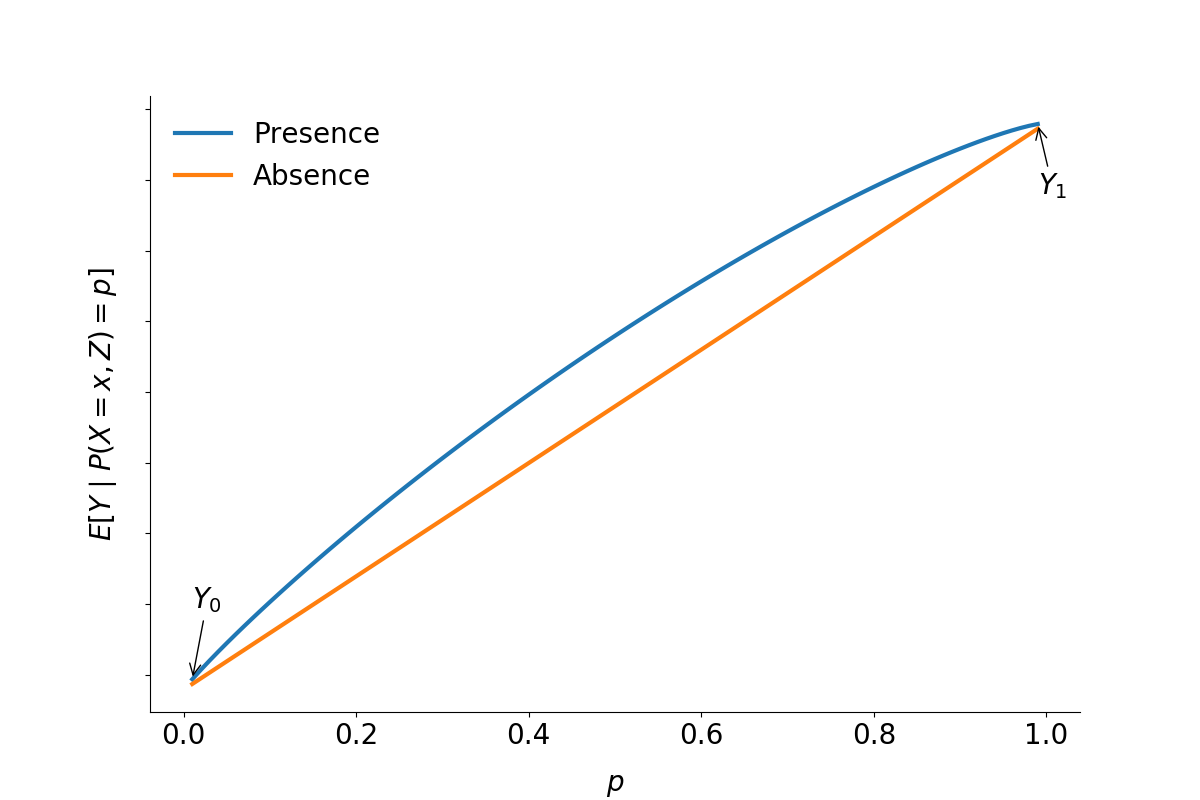
\includegraphics{fig-eh-conditional-expectation.png}}
\end{figure}

\end{frame}



%\begin{frame}
 %\frametitle{Parameters of Interest}
%\subsection{Parameters of Interest}\label{parameters-of-interest}

%\end{frame}

\begin{frame}
%\subsubsection{Conventional TreatmentEffects}\label{conventional-treatment-effects}
\frametitle{Conventional Treatment Effects}

\begin{align*}
B^{ATE} & = E[Y_1 - Y_0 ]\\
B^{TT} & = E[Y_1 - Y_0 \mid D = 1]\\
B^{TUT} & = E[Y_1 - Y_0 \mid D = 0]\\
\end{align*}

\(\Rightarrow\) correspond to \emph{extreme} policy alternatives

\end{frame}


\begin{frame}
%\subsubsection{Selection Problem}\label{selection-problem}
\frametitle{Selection Problem}

\begin{align*}
E[Y\mid D = 1] - E[Y\mid D = 0] & = \underbrace{E[Y_1 - Y_0]}_{B^{ATE}} \\
	 							& + \underbrace{E[Y_1 - Y_0 \mid D = 1] - E[Y_1 - Y_0]}_{\text{Sorting Gain}} \\
								& + \underbrace{E[Y_0\mid D = 1] - E[Y_0 \mid D = 0]}_{\text{Selection Bias}}
\end{align*}

\end{frame}


\begin{frame}
%\subsubsection{Selection Problem}\label{selection-problem}
\frametitle{Selection Problem}

\begin{align*}
E[Y\mid D = 1] - E[Y\mid D = 0] & = \underbrace{E[Y_1 - Y_0\mid D = 1]}_{B^{TT}} \\
& + \underbrace{E[Y_0\mid D= 1]- E[Y_0 \mid D = 0]}_{\text{Selection Bias}}
\end{align*}

\(\Rightarrow\) the bias depends on the parameter of interest

\end{frame}


\begin{frame}
%\frametitle{Treatment Effects with Essential Heterogeneity}

\begin{figure}[htp]\centering
	\caption{Treatment Effects with Essential Heterogeneity}\label{Treatment Effects Conventional}\scalebox{0.35}{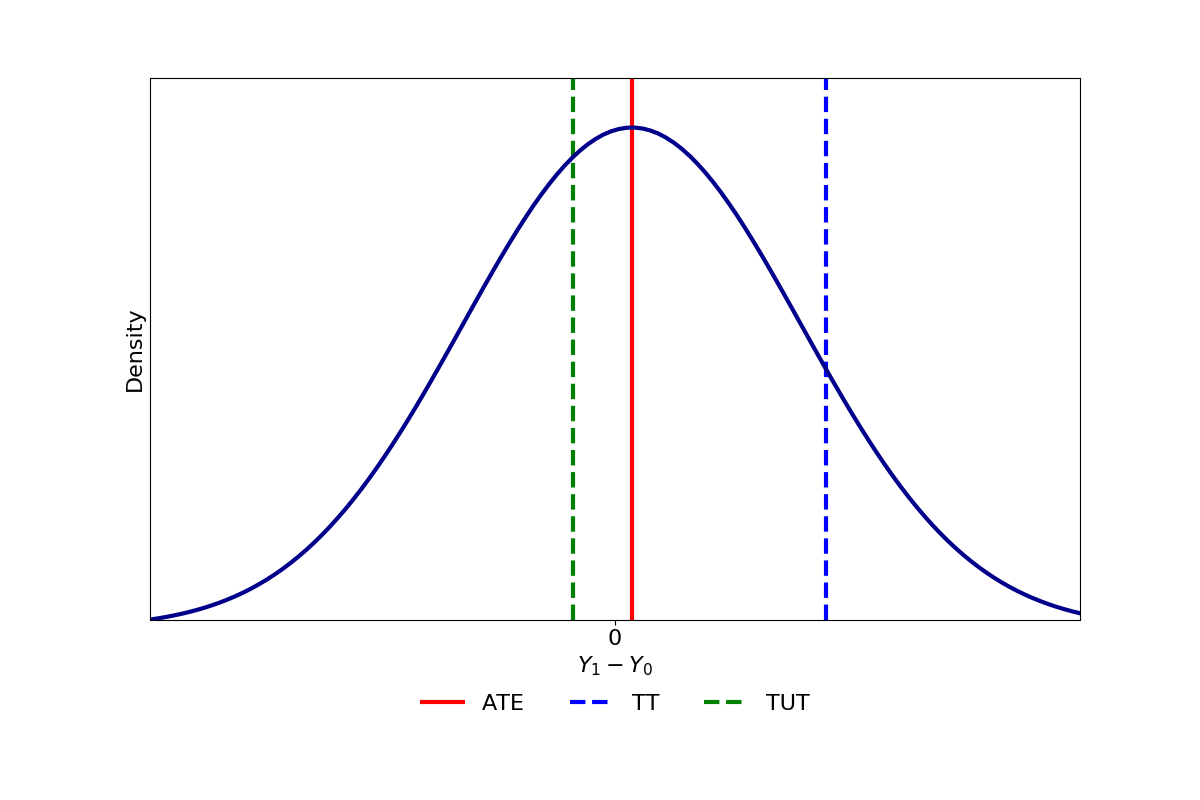
\includegraphics{fig-treatment-effects-conventional.png}}
\end{figure}

\end{frame}


\begin{frame}
%\frametitle{Treatment Effects without Essential Heterogeneity}

\begin{figure}[htp]\centering
	\caption{Treatment Effects without Essential Heterogeneity}\label{Treatment Effects Without Essential Heterogeneity}\scalebox{0.35}
	{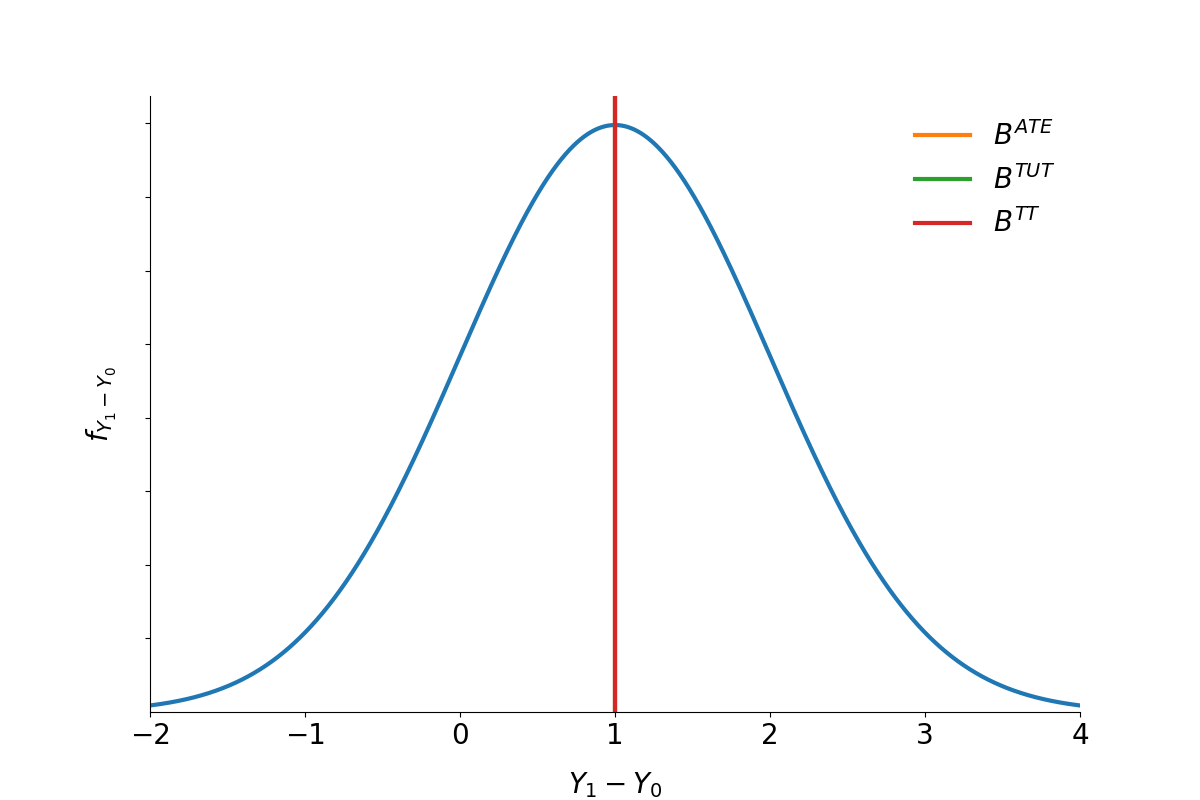
\includegraphics{fig-treatment-effects-without-eh.png}}
\end{figure}

\end{frame}


\begin{frame}
    \subsubsection{Policy - Relevant Average Treatment Effect}\label{policy---relevant-average-treatment-effect}
\frametitle{Policy - Relevant Average Treatment Effect}

\textbf{Observed Outcomes}

\begin{align*}
Y_B = D_B Y_1 + (1 - D_B) Y_0 \\
Y_A = D_A Y_1 + (1 - D_A) Y_0 \\
\end{align*}

\textbf{Effect of Policy}

\begin{align*}
B^{PRTE} = \frac{1}{E[D_A] - E[D_B]} (E[Y_A] - E[Y_B])
\end{align*}

\end{frame}


\begin{frame}
    \subsubsection{Marginal Benefit of Treatment}\label{marginal-benefit-of-treatment}
\frametitle{Marginal Benefit of Treatment}

\begin{align*}
B^{MTE}(x, u_S) = E [Y_1 - Y_0 \mid X = x, U_S = u_S]
\end{align*}

\textbf{Intuition:} Mean gross return to treatment for persons at
quantile \(u_S\) of the first-stage unobservable \(V\).

\end{frame}


\begin{frame}
%\frametitle{Treatment Effects with Essential Heterogeneity}

\begin{figure}[htp]\centering
	\caption{Treatment Effects: Margin of Indifference}\label{Margin Indifference}\scalebox{0.35}
	{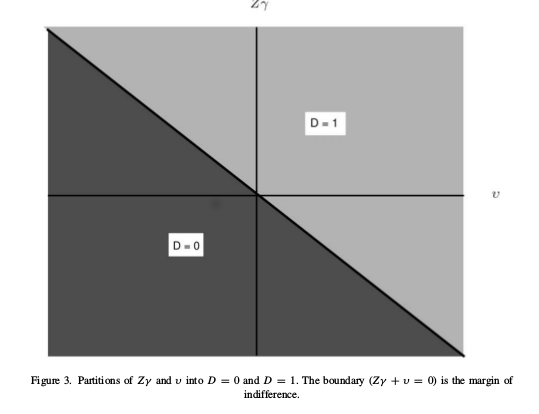
\includegraphics{fig-margin-indifference.png}}
\end{figure}

\end{frame}


\begin{frame}
%\frametitle{Treatment Effects with Essential Heterogeneity}

\begin{figure}[htp]\centering
	\caption{Marginal Effect of Heterogeneity}\label{Marginal Effect of Heterogeneity}\scalebox{0.35}
	{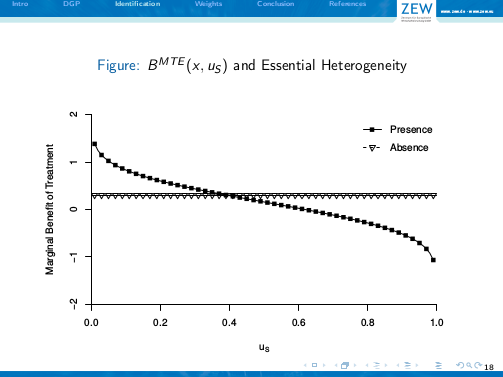
\includegraphics{fig-eh-marginal-effect.png}}
\end{figure}

\end{frame}


\begin{frame}
%\subsubsection{Effects of Treatment as Weighted Averages}\label{effects-of-treatment-as-weighted-averages}
\frametitle{Effects of Treatment as Weighted Averages}

Parameter \(\Delta_j\), can be written as a weighted average of the
\(B^{MTE}(x, u_S)\).

\begin{align*}
\Delta_j(x) = \int_0^1 B^{MTE}(x, u_S) \omega^j(x, u_S) du_S,
\end{align*}

where the weights \(\omega^j(x, u_S)\) are specific to parameter \(j\)
and integrate to one.
\end{frame}

\begin{frame}
\frametitle{Effects of Treatment as Weighted Averages}
\textbf{Weights}

\begin{align*}
 \omega^{ATE}(x, u_S) & = 1 \\
 \omega^{TT}(x, u_S) & = \frac{1 - F_{P\mid X=x}(u_S)}{E[P \mid X = x]}\\
 \omega^{TUT}(x, u_S) & = \frac{F_{P\mid X=x}(u_S)}{E[1 - P \mid X = x]}
\end{align*}

\end{frame}


\begin{frame}
%\frametitle{Effects of Treatment as Weighted Averages}

\begin{figure}[htp]\centering
	\caption{Effects of Treatment as Weighted Averages}\label{Effects of Treatment as Weighted Averages}\scalebox{0.35}
	{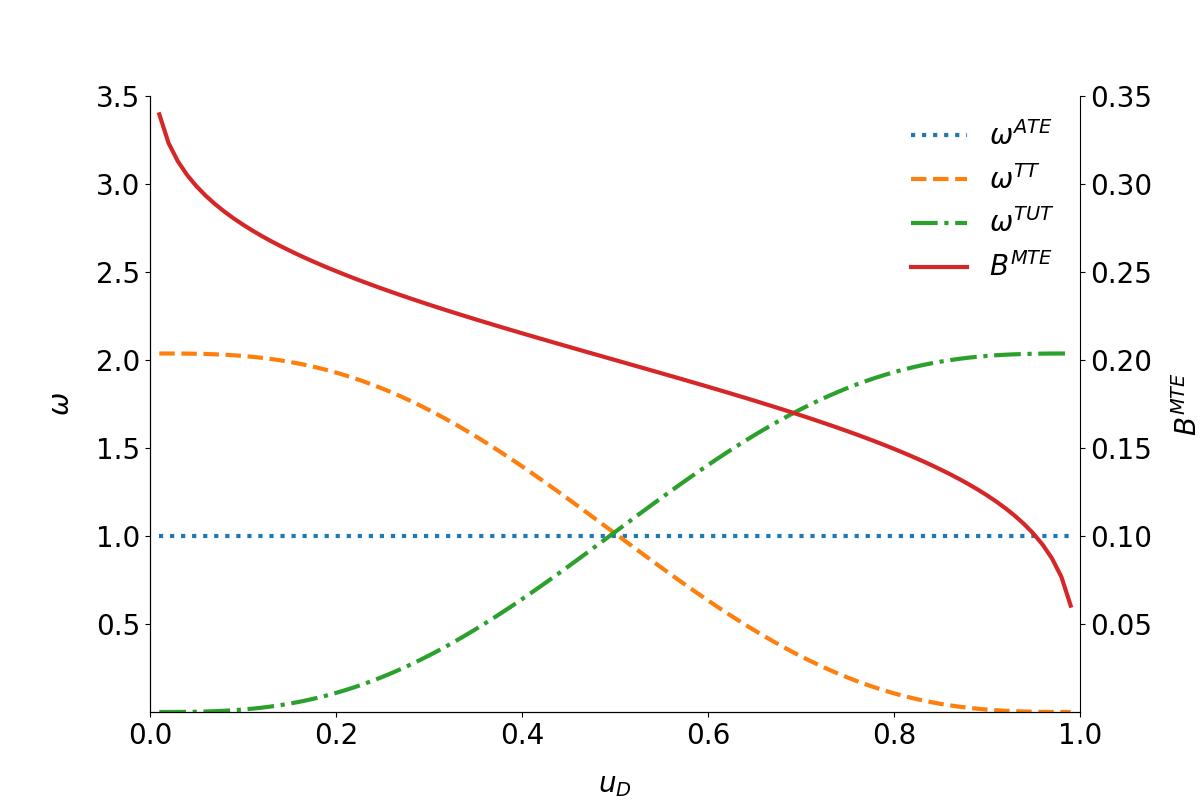
\includegraphics{fig-weights-marginal-effect.png}}
\end{figure}

\end{frame}


\begin{frame}
%\subsubsection{Local Average Treatment Effect}\label{local-average-treatment-effect}
\frametitle{Local Average Treatment Effect}

\begin{itemize}
\item \textbf{Local Average Treatment Effect:} Average effect for those induced
to change treatment because of a change in the instrument.
\(\Rightarrow\) instrument-dependet parameter

\item \textbf{Marginal Treatment Effect:} Average effect for those individuals
with a given unobserved desire to receive treatment.\\
\(\Rightarrow\) deep economic parameter
\end{itemize}

    \begin{align*}
B^{LATE} = \frac{E(Y\mid Z = z) - E[Y \mid Z = z^\prime]}{P(z) - P(z^\prime)}
\end{align*}

\begin{align*}
B^{LATE}(x, u_S, u_{S^\prime}) = \frac{1}{u_S - u_{S^\prime}} \int_{u_S}^{u_{S^\prime}} B^{MTE}(x, u) du,
\end{align*}

\end{frame}


\begin{frame}
%\frametitle{Local Average Treatment Effect}

\begin{figure}[htp]\centering
	\caption{Local Average Treatment Effect}\label{Local Average Treatment}\scalebox{0.35}
	{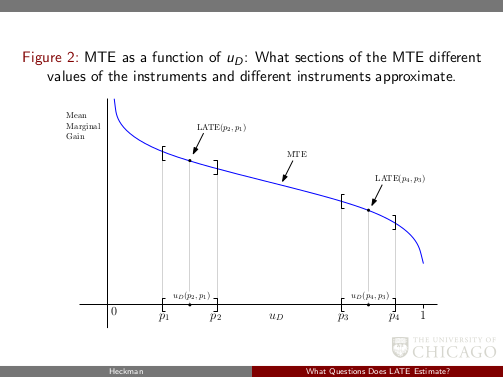
\includegraphics{fig-local-average-treatment.png}}
\end{figure}

\end{frame}


\begin{frame}
%\subsubsection{Distributional Effects of Treatment}\label{distributional-effects-of-treatment}
\frametitle{Distributional Effects of Treatment}

\begin{itemize}
\item
  Marginal Distribution of Benefits
\item
  Joint Distribution of Potential Outcomes
\item
  Joint Distribution of Benefits and Surplus
\end{itemize}
\end{frame}


\begin{frame}

\begin{figure}[htp]\centering
	\caption{Distribution of Benefits}\label{Treatment Effects Benefits}\scalebox{0.35}
	{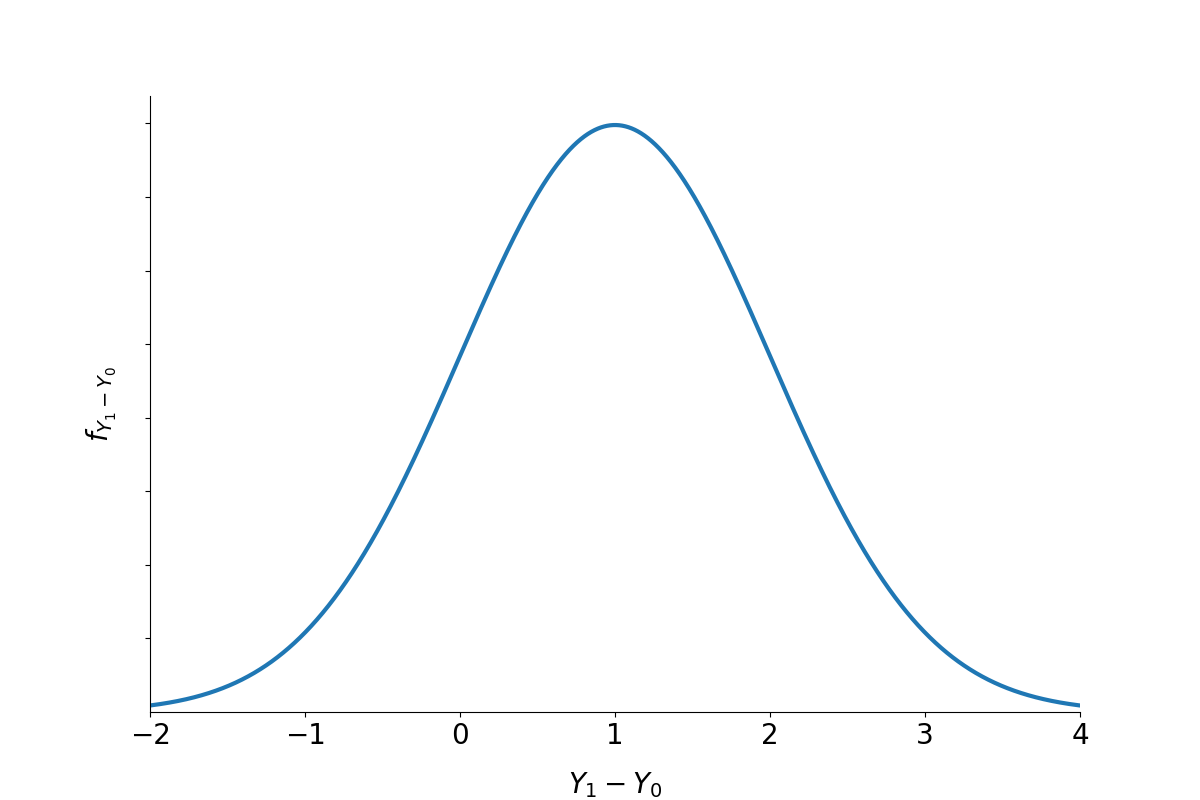
\includegraphics{fig-treatment-effects-benefits.png}}
\end{figure}

\end{frame}


\begin{frame}
%\frametitle{Distributional Effects of Treatment}

\begin{figure}[htp]\centering
	\caption{Joint Distribution of Potential Outcomes}\label{Treatment Effects Benefits}\scalebox{0.80}
	{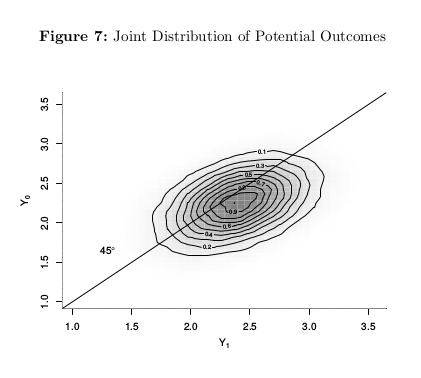
\includegraphics{fig-distribution-potential.png}}
\end{figure}

\end{frame}


\begin{frame}
%\frametitle{Distributional Effects of Treatment}

\begin{figure}[htp]\centering
	\caption{Joint Distribution of Surplus and Benefits}\label{Treatment Effects Benefits}\scalebox{0.80}
	{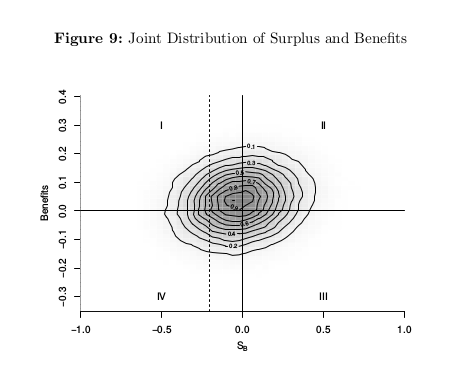
\includegraphics{fig-distribution-surplus.png}}
\end{figure}

\end{frame}


\begin{frame}
\frametitle{Teaching Tool}

\begin{figure}[htp]\centering
	
\includegraphics[width=\textwidth]{fig-online-documentation.png}
%\caption{Teaching Tool}\label{Teaching Tool}
%\scalebox{0.18}{
\includegraphics{fig-online-documentation.png}}
\end{figure}

\end{frame}



    % Add a bibliography block to the postdoc


%!TEX root = ../main.tex
\beginbackup
%\appendix
%\begin{frame}\begin{center}
%\LARGE\textbf{Appendix}
%\end{center}\end{frame}

%------------------------------------------------------------------------------
%------------------------------------------------------------------------------
\begin{frame}\begin{center}
\LARGE\textit{References}
\end{center}\end{frame}
%------------------------------------------------------------------------------
%------------------------------------------------------------------------------
\newgeometry{margin=1cm}
\begin{frame}[allowframebreaks]\frametitle{}

\nocite{Abbring.2007,Carneiro.2003,Carneiro.2011,Heckman.2001g,Heckman.2008a,Heckman.1997,Heckman.2006d,Heckman.2001d,Heckman.2001e,Heckman.2005e,Heckman.2007e,Heckman.2007f,Roy.1951}

\bibliographystyle{apalike}
\bibliography{../../submodules/bibliography/literature}


\end{frame}

\backupend
\end{document}
